\chapter{Controllo $H_\infty$: baseline e revisione mirata}
\label{cap:hinf}
\section{Obiettivo energetico e mappe della retroazione}
Il controllo $H_\infty$ cerca un regolatore che limiti il peggiore guadagno
delle mappe di interesse. Per una matrice di trasferimento stabile $F$,
\[
\|F\|_\infty=\sup_{\omega\in\mathbb R}\bar\sigma(F(j\omega))
=\sup_{0<\|w\|_2<\infty}\frac{\|z\|_2}{\|w\|_2},\qquad z=Fw.
\]
Si considera quindi la peggiore frequenza e la peggiore direzione MIMO
dell'ingresso, non la media dei due giunti. L'interpretazione energetica
riguarda ingressi a energia finita. Un gradino permanente non è in $L_2$:
settling, overshoot e picco istantaneo di coppia devono essere verificati
separatamente, non dedotti automaticamente dalla norma.

Per la pianta M3, $G:u\mapsto q$ ha dimensione $2\times2$, 14 stati,
ingressi in N m e uscite in rad. Il regolatore riceve $e=r-q$ e produce
$u=Ke$. Definiamo le mappe all'uscita
\[
S=(I+GK)^{-1},\qquad
T=GK(I+GK)^{-1}=I-S,\qquad
KS=K(I+GK)^{-1}.
\]
$S$ collega riferimento ed errore, $T$ riferimento e posizione,
$KS$ riferimento e comando. Un rumore additivo di misura si trasmette
alla posizione mediante $-T$ e al comando mediante $-KS$.
Per la coppia disturbante lato link, invece, la mappa fisica è
$SG_d$: non basta chiamare $S$ la risposta a qualsiasi disturbo.

LQG e $H_\infty$ rispondono a problemi diversi. M6 impiega una stima
dello stato basata su $q,\theta$ e ipotesi statistiche sui rumori;
la sintesi qui studiata utilizza soltanto i due errori di posizione $r-q$
e minimizza un criterio frequenziale worst-case. Non riutilizza $K$ o $L$
di M6 e non dispone automaticamente delle stesse prestazioni.

\section{Mixed sensitivity: pesi e sintesi con mixsyn}
M9 risolve, sulla pianta fisica M3,
\[
\min_K\left\|\begin{bmatrix}W_1S\\W_2KS\end{bmatrix}\right\|_\infty
\]
mediante \texttt{mixsyn(G,W1,W2,[])}. I pesi seguenti sono quelli
selezionati dalla revisione del §8.4 e salvati in M5.
I target temporali del Capitolo 6 rimangono invariati: rilassare
l'inviluppo pesato non equivale a dichiarare ammissibile un errore
statico superiore al 5\%.

\subsection{Peso sulla sensibilità}
Con $S=(I+GK)^{-1}$ adottiamo
\[
W_1(s)=\frac{s/M_s+\omega_{W1}}{s+\omega_{W1}A_s},\qquad
A_s=0.15,\quad M_s=2.5.
\]
Ponendo $s=0$ si ottiene
\[
W_1(0)=\frac{1}{A_s}=6.\overline{6}.
\]
Pertanto $\|W_1S\|_\infty<1$ richiede una sensitivity dell'ordine del 15\% alle basse frequenze. Dividendo numeratore e denominatore per $s$ e passando al limite,
\[
W_1(\infty)=\frac{1}{M_s}=0.4.
\]
Il vincolo lascia quindi un picco di sensitivity dell'ordine di $M_s=2.5$; $\omega_{W1}$ colloca la transizione tra accuratezza statica e roll-off.

La frequenza a modulo unitario non coincide esattamente con $\omega_{W1}$:
\[
\omega_{|W_1|=1}=\omega_{W1}
\sqrt{\frac{1-A_s^2}{1-1/M_s^2}}=\RevHinfCrossover\ \mathrm{rad/s}.
\]
Polo e zero sono rispettivamente 1.2 e 20 rad/s.

La lettura del peso deve essere fatta attraverso il suo inverso. Se $\|W_1S\|_\infty<1$, allora $\bar\sigma(S)<1/|W_1|$: a bassa frequenza l'errore deve essere piccolo, nella zona di transizione si fissa la rapidità desiderata e ad alta frequenza il vincolo si rilassa. Non si tenta quindi di rendere $S$ piccolo a tutte le frequenze, cosa incompatibile con il roll-off e con i limiti di robustezza.

\subsection{Peso sul comando}
Il peso agisce direttamente sulla coppia fisica:
\[
W_2(s)=k_u\frac{s+\omega_U}{s/\alpha+\omega_U},\qquad
k_u=0.05,\quad \omega_U=60\ \mathrm{rad/s},\quad\alpha=6.
\]
A bassa frequenza $W_2(0)=k_u=0.05$; ad alta frequenza tende
a $\alpha k_u=0.30$. La penalizzazione aumenta di un fattore sei:
lo zero è a 60 rad/s, il polo a 360 rad/s. Questi sono parametri
di progetto, non una curva coppia--velocità fornita dalla traccia.

Anche qui l'inviluppo desiderato è $1/|W_2|$: il suo valore numerico
passa da 20 a $10/3$. Esso limita la mappa $KS:r\mapsto u$, cioè
il guadagno energetico del comando rispetto al riferimento nelle
coordinate SI adottate, non il picco istantaneo assoluto di coppia.
Un gradino di 5 gradi non è un ingresso unitario e una norma frequenziale
non è una saturazione nel tempo. La scala $u_{scale}=12$ N m
rimane utilizzata nelle metriche comparative, ma non definisce più
$W_2$. Poiché il modulo del peso resta inferiore a uno, non esiste
un suo crossover unitario.

\subsection{Implementazione e interpretazione}
I pesi MIMO sono due copie diagonali dei filtri SISO e M9/M10 non usano
$W_3$. Il valore uno separa soddisfacimento e violazione del profilo
pesato. I test verificano stabilità, properness, dimensioni e asintoti.
La scelta dei pesi è distinta dalla valutazione: dopo la selezione
i pesi restano fissi in ogni sintesi e analisi successiva.
Le specifiche di tracking non sono modificate quando una sintesi
produce $\gamma>1$.

La stessa M5 fornisce al costo LQR ampiezza, scala di velocità e
deformazione, senza rendere equivalenti LQR e mixed sensitivity.
In particolare $\omega_B=12$ rimane la scala generale di banda,
mentre $\omega_{W1}=8$ colloca la transizione del peso: confondere
i due parametri introdurrebbe un retuning non richiesto di $Q$.

\begin{figure}[htbp]\centering
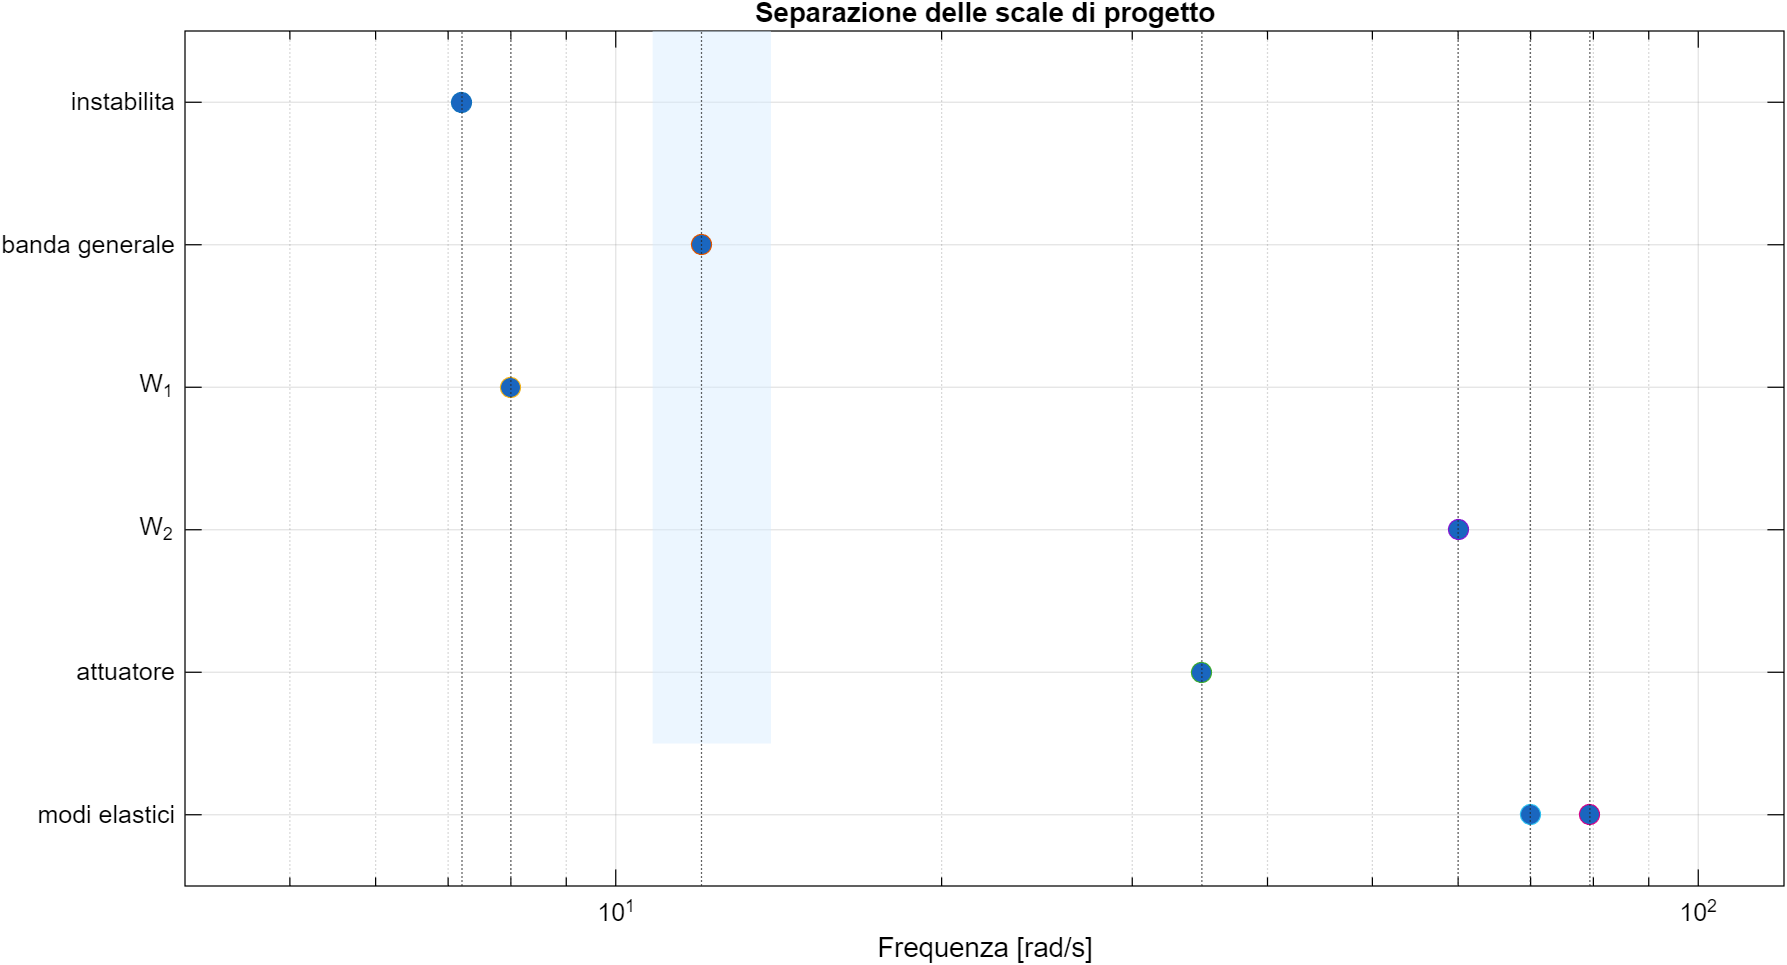
\includegraphics[width=0.79\textwidth]{figures/m5_spec_frequency_map.png}
\caption{Scale dinamiche e distinzione fra banda generale, transizione di
$W_1$ e inizio della crescita di $W_2$.}\label{fig:m5-map}
\end{figure}

\section{M10: pianta generalizzata e Lower LFT}
M10 costruisce invece esplicitamente, con \texttt{connect} e
\texttt{sumblk}, i segnali
$e=r-q$, $z_1=W_1e$, $z_2=W_2u$:
\[
\begin{bmatrix}z_1\\z_2\\e\end{bmatrix}
=
\underbrace{\begin{bmatrix}
W_1&-W_1G\\0&W_2\\I&-G
\end{bmatrix}}_{P}
\begin{bmatrix}r\\u\end{bmatrix}.
\]
Qui $w=r\in\mathbb R^2$ è l'ingresso esogeno,
$z=[z_1^T,z_2^T]^T\in\mathbb R^4$ l'uscita prestazionale,
$y=e\in\mathbb R^2$ la misura fornita al controllore e
$u\in\mathbb R^2$ il comando. Nell'ordine richiesto da
\texttt{hinfsyn}, le misure sono le ultime uscite e i comandi gli
ultimi ingressi. La pianta è quindi $6\times4$.

Partizionando $P$ secondo $[z;y]$ e $[w;u]$, la lower LFT è
\[
F_\ell(P,K)=P_{11}+P_{12}K(I-P_{22}K)^{-1}P_{21}.
\]
Il segno negativo della retroazione è già contenuto in $P_{22}=-G$:
non va aggiunto un secondo cambio di segno.
La chiamata \texttt{hinfsyn(P,2,2)} e \texttt{mixsyn(G,W1,W2,[])}
rappresentano lo stesso problema quando pesi e segnali coincidono.
M10 ne verifica l'equivalenza, ottenendo ordine \KhinfOrder\
e $\gamma=\HinfsynGamma$.

\begin{figure}[htbp]\centering
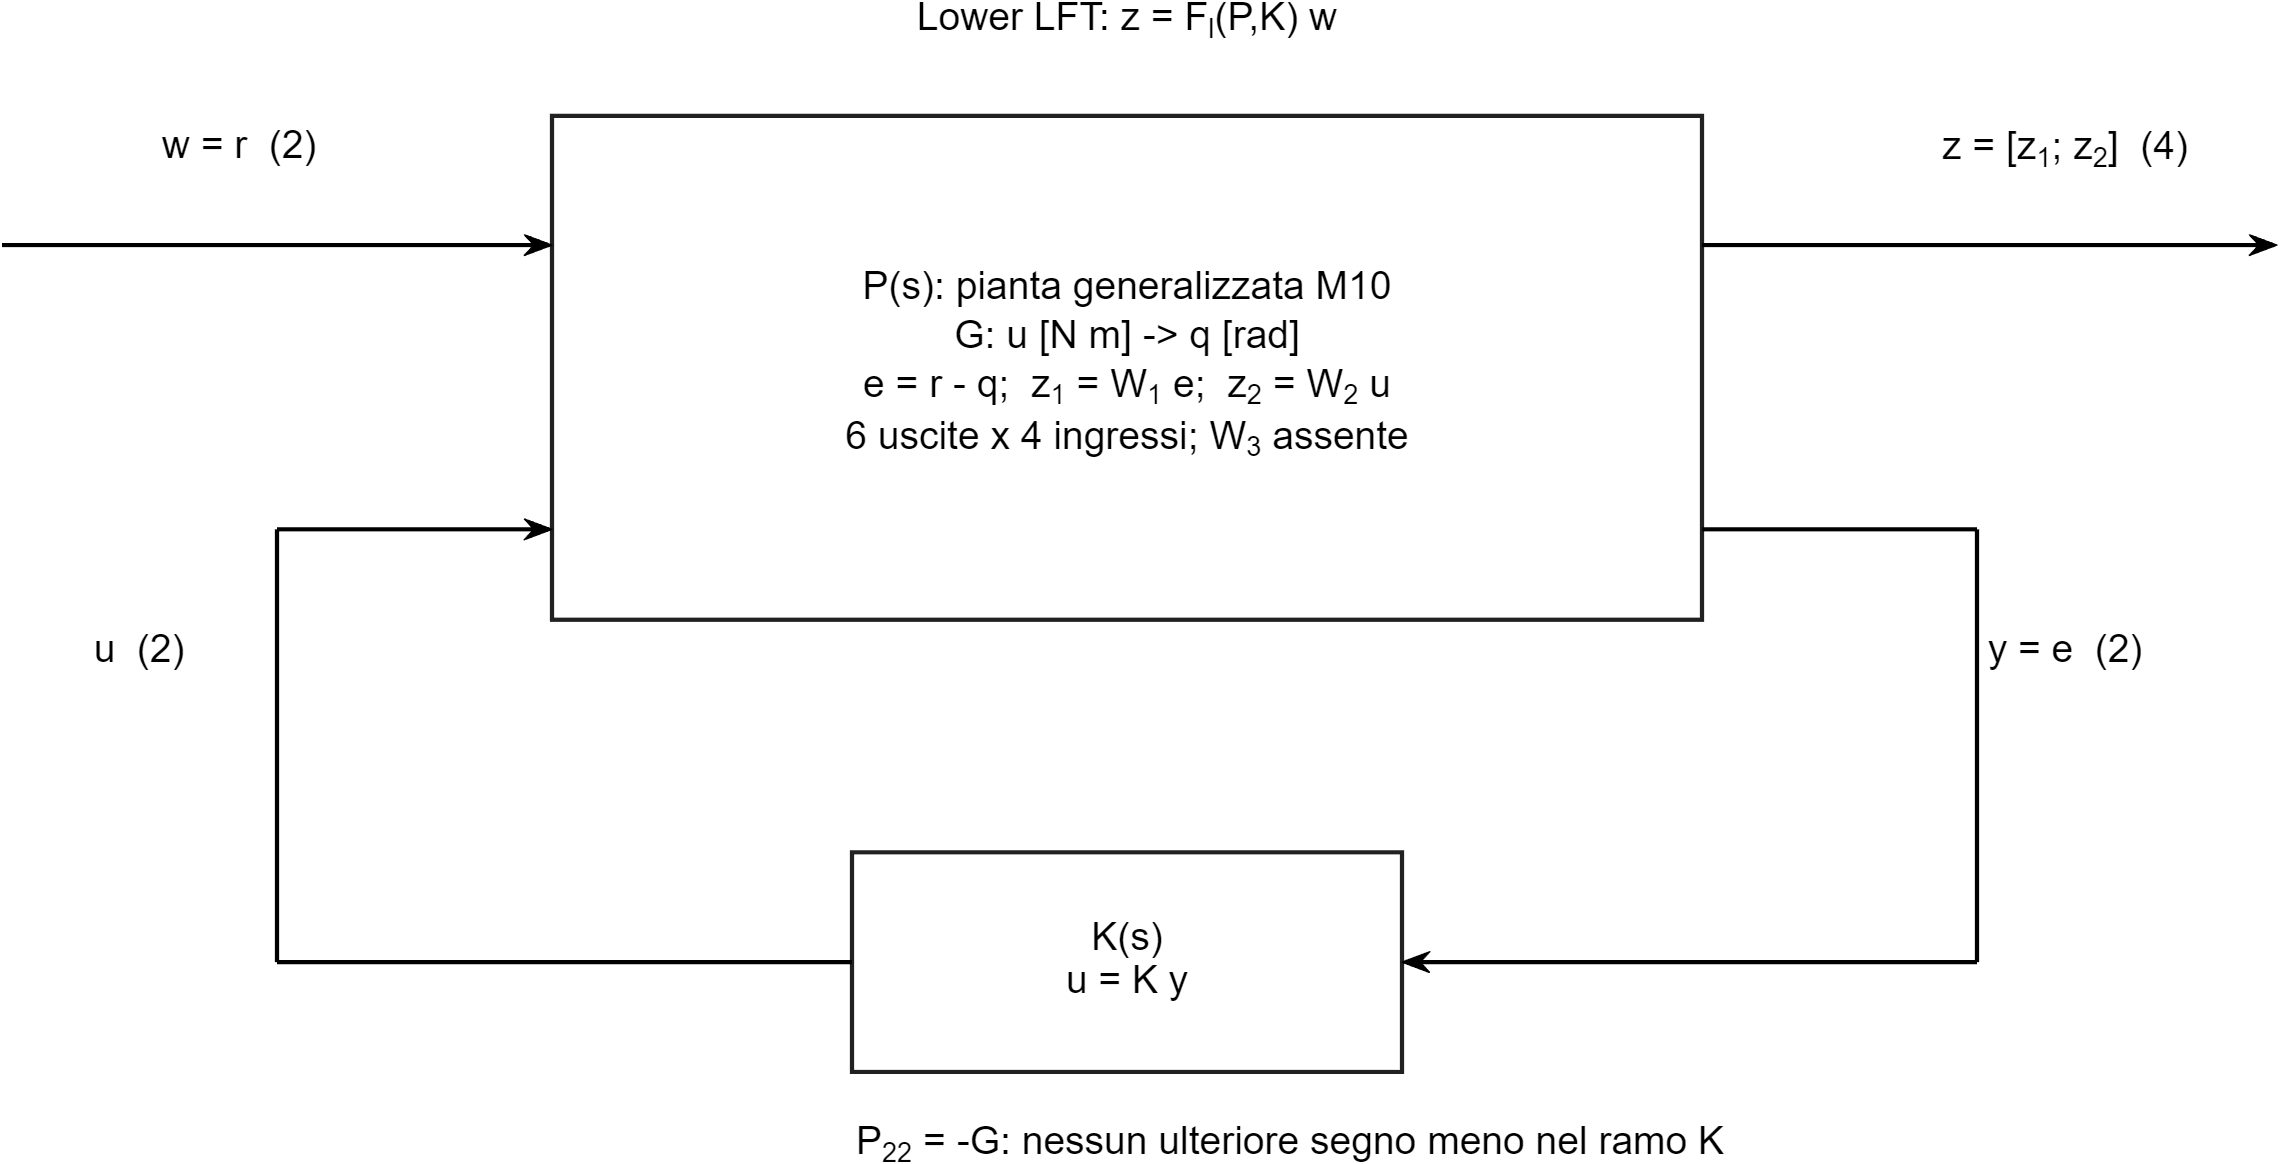
\includegraphics[width=0.95\textwidth]{figures/m10_lower_lft_block_diagram.png}
\caption{Lower LFT realmente impiegata in M10. Il ramo inferiore chiude
$y=e$ sul controllore e riporta $u=Ky$ alla pianta generalizzata.
Sono presenti soltanto i canali $W_1e$ e $W_2u$.}
\label{fig:m10-lower-lft}
\end{figure}
Lo schema è generato da \path{plot_m10_lower_lft_diagram.m}, che
verifica dimensioni e partizioni dell'artifact M10 prima dell'esportazione.
Non compaiono disturbi o rumori come ingressi di sintesi: sono scenari
della successiva validazione.

\begin{figure}[htbp]\centering
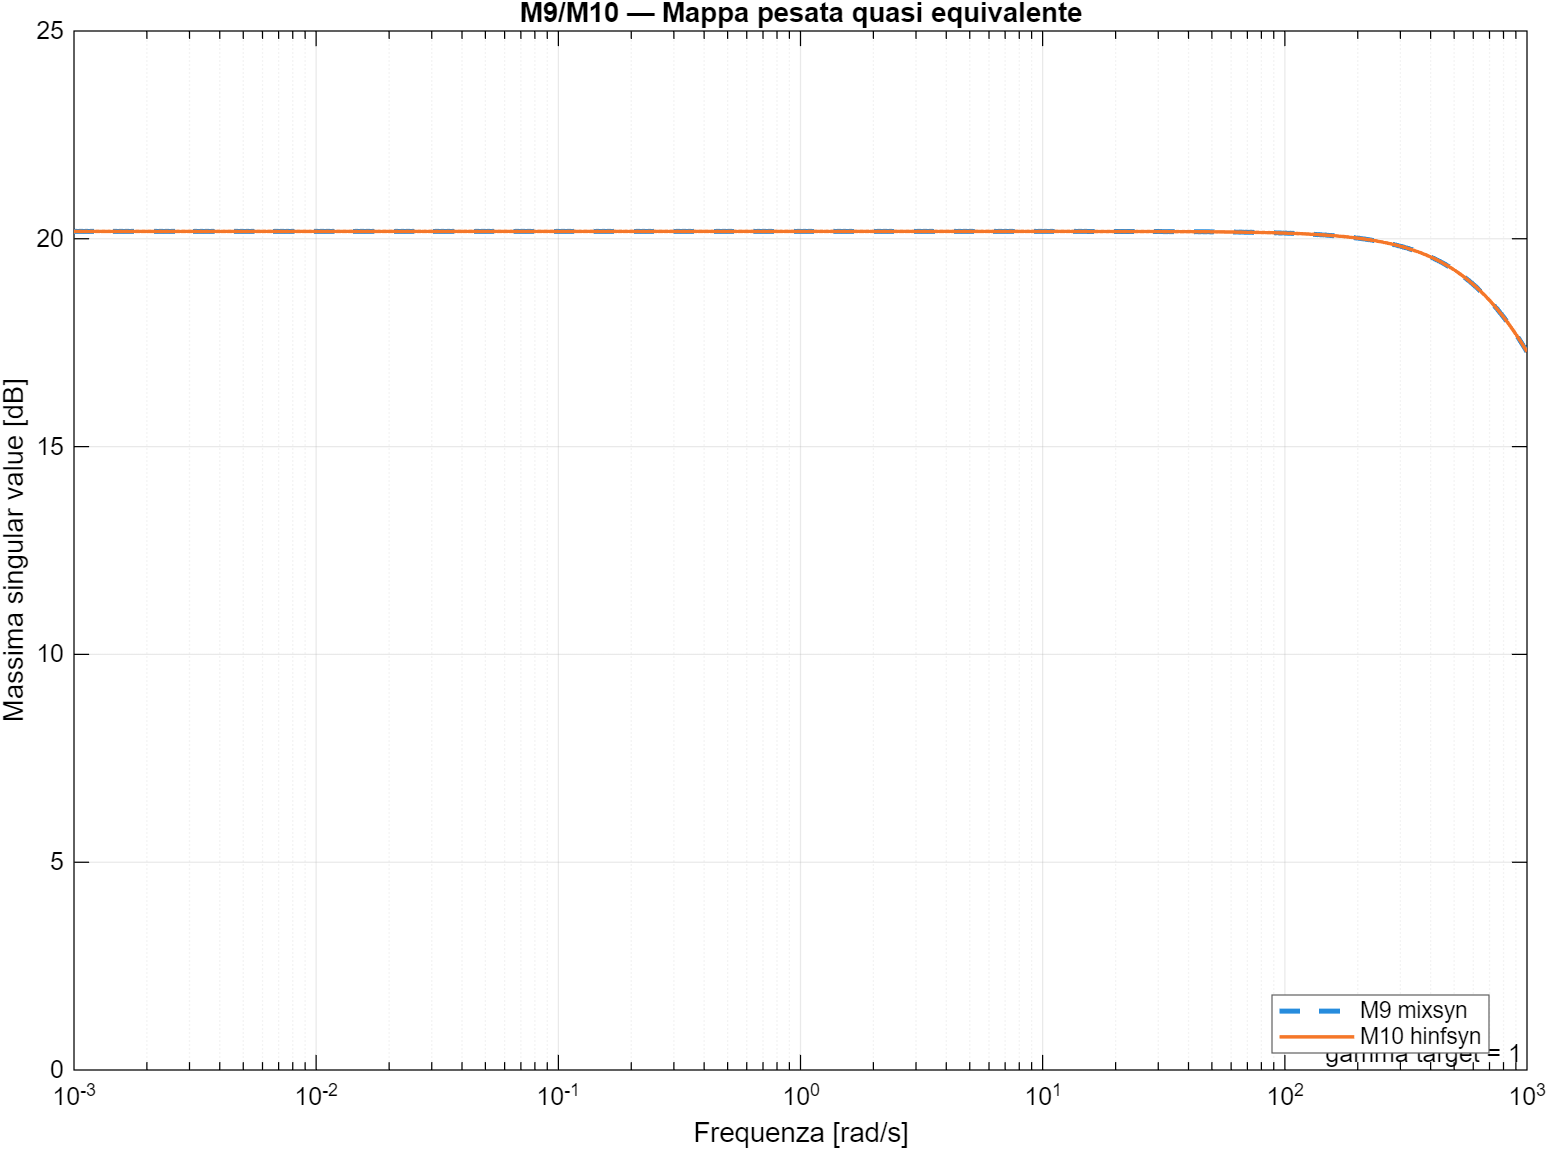
\includegraphics[width=0.88\textwidth]{figures/m10_weighted_comparison_m9.png}
\caption{M9/M10 con i nuovi pesi: la sovrapposizione verifica
l'equivalenza delle interconnessioni, non il soddisfacimento del target uno.}
\label{fig:m10-weighted}
\end{figure}

\section{Revisione diretta dei pesi}
La baseline a due pesi usava
\[
W_{1,0}=\frac{s/2+12}{s+0.6}I_2,\qquad
W_{2,0}=\frac1{12}\frac{s+30}{s/6+30}I_2.
\]
I contributi erano circa $10.128$ per $W_1S$ e $10.185$ per $W_2KS$,
con $\gamma=10.207$. Entrambi gli inviluppi erano violati.
A 12 rad/s i valori singolari di $G$ sono circa $0.1713$ e $0.0101$
rad/(N m): la direzione meno efficace richiede più comando.
I poli instabili, il ritardo e la flessibilità limitano il compromesso.
La revisione modifica direttamente i filtri, lasciando invariati
$G:u\,[\mathrm{N\,m}]\mapsto q\,[\mathrm{rad}]$ e tutti i target temporali.

\subsection{Una incompatibilità verificabile prima del retuning}
Con pesi scalari replicati sui due giunti, poniamo
$a=|W_{1,\mathrm{siso}}(j\omega)|$,
$b=|W_{2,\mathrm{siso}}(j\omega)|$ e
$g=\underline\sigma(G(j\omega))$. Poiché $S+GKS=I$, persino
rilassando il problema e scegliendo liberamente il comando complesso
a ogni frequenza, il costo nella direzione meno efficace non può
scendere sotto
\[
\gamma\ \geq\
\sup_\omega \frac{a(\omega)b(\omega)}
{\sqrt{b(\omega)^2+a(\omega)^2g(\omega)^2}}.
\]
Il limite deriva dalla minimizzazione quadratica puntuale di
$a^2|1-gv|^2+b^2|v|^2$ rispetto al comando $v$.
Non impone causalità o stabilità del controllore: è una condizione
necessaria, non una formula per il controllore ottimo.

Con i pesi originali il valore calcolato sulla griglia è almeno
$1.645$ a circa $5.754$ rad/s. Esiste quindi già un conflitto fra
i due inviluppi che esclude $\gamma<1$, indipendentemente dall'algoritmo
di sintesi. Non spiega da solo l'intero valore $10.207$:
i vincoli dinamici e di stabilità interna rendono il problema completo
più restrittivo del rilassamento puntuale.

\subsection{Ricerca limitata e motivazione dei parametri}
Stage A esplora otto combinazioni:
\[
\omega_{W1}\in\{6,8\},\quad A_s\in\{0.10,0.15\},\quad
M_s\in\{2.5,3\}.
\]
Abbassare la transizione riduce la richiesta di accuratezza in frequenza;
aumentare $A_s$ riduce il guadagno DC del peso e aumentare $M_s$
rilassa l'inviluppo ad alta frequenza. Sono livelli progettuali
semplici, non valori determinati univocamente dalla fisica.
Stage A conserva il $W_2$ effettivo della baseline, con
$k_u=1/12$ e $\omega_U=30$ rad/s.

Non essendoci PASS e risultando $W_2KS$ dominante nei due migliori
candidati, Stage B considera soltanto quei due $W_1$, con
$k_u\in\{0.05,0.07\}$ e $\omega_U=60$ rad/s.
Il guadagno più basso penalizza meno il comando; il nuovo zero sposta
l'inizio della crescita. Si eseguono quattro ulteriori sintesi:
12 candidati totali, senza ricerca casuale e senza cambiare le soglie.
Il limite previsto di due PASS avrebbe interrotto Stage A; un PASS
avrebbe arrestato Stage B. Nessuno si è verificato.

Lo studio aggiuntivo conserva il terzo peso già presente:
\[
W_3(s)=\frac{s/40+0.1}{s/200+1}I_2.
\]
Il guadagno DC 0.1 e quello HF 5 rappresentano un obiettivo nominale
di roll-off e attenuazione del rumore; 40 rad/s richiama la frequenza
naturale dell'attuatore. Non sono dati di identificazione.
$W_3$ non domina il compromesso selezionato, quindi non vengono
esplorate alternative. M9/M10/M11 restano invece a due pesi:
la configurazione selezionata trasferisce loro solo $W_1,W_2$.

Il peso d'incertezza $W_I$ M4 agisce all'ingresso; la relativa
complementarità $T_i=KG(I+KG)^{-1}$ non coincide in generale con
$T=GK(I+GK)^{-1}$. Il peso nominale $W_3$ non sostituisce pertanto
la successiva $\mu$-analysis.

\begin{table}[htbp]\centering\small
\begin{tabular}{lp{2.2cm}p{2.2cm}p{6.3cm}}\toprule
Parametro & Iniziale & Selezionato & Significato\\\midrule
$\omega_{W1}$ & 12 & 8 rad/s & Transizione meno aggressiva, distinta da $\omega_B$\\
$A_s$ & 0.05 & 0.15 & Minore guadagno DC del peso, target statico invariato\\
$M_s$ & 2 & 2.5 & Inviluppo di sensibilità meno restrittivo\\
$k_u$ & $1/12$ & 0.05 & Minore penalizzazione diretta del comando\\
$\omega_U$ & 30 & 60 rad/s & Crescita del peso spostata in frequenza\\
$W_3$ studio & $\omega_T=40$ & invariato & Non dominante; assente nella produzione M10\\\bottomrule
\end{tabular}
\caption{Parametri di progetto selezionati, non nuovi limiti fisici.}
\label{tab:hinf-pesi-nuovi}\end{table}

\subsection{Selezione e ricostruzione indipendente}
Ogni candidato è verificato sulla matrice completa plant--controller,
sulle norme componenti e sullo stack, e su due gradini separati da
5 gradi per 12 s. Il PASS richiede stabilità, $\gamma<1$ e tutti i
target di settling, overshoot ed errore statico.
Fra i candidati stabili l'ordinamento lessicografico considera
$\gamma<1$, numero di target temporali violati, massimo rapporto
metrica/target, picco relativo di comando, cross-coupling e infine $\gamma$.
Il compromesso ID 10 non viene dichiarato conforme.

Per lo studio a tre pesi, nelle medesime coordinate fisiche,
\[
P_3=\begin{bmatrix}W_1&-W_1G\\0&W_2\\0&W_3G\\I&-G\end{bmatrix},
\qquad F_\ell(P_3,K)=\begin{bmatrix}W_1S\\W_2KS\\W_3T\end{bmatrix}.
\]
La pianta $8\times4$ è verificata mediante formula a blocchi,
\texttt{connect}, \texttt{augw} e ricostruzione della lower LFT.
Questo non altera la pianta $6\times4$ di M10.

\section{M11: sintesi strutturata con i pesi selezionati}
Il controllore full-order non impone una struttura a basso ordine:
M10 ha ordine 18; lo studio a tre pesi ha ordine 20 perché aggiunge
due stati di peso. Un ordine maggiore aumenta la libertà dinamica,
non garantisce automaticamente prestazioni conformi o robustezza.

M11 viene rigenerata una volta sul nuovo problema a due pesi.
Comprende guadagno statico MIMO, due PI decentralizzati, due PID
filtrati e tre strutture MIMO di ordine 2, 4, 6, con cinque partenze
per famiglia. Le configurazioni e i criteri restano invariati.
A0/A1 non producono soluzioni valide stabili; A2 non produce chiusure
stabili. A3/A4/A5 producono cinque chiusure stabili ciascuna.
L'aumento di ordine riduce il divario dal full-order, ma nessuna
famiglia soddisfa l'intero profilo. Le partenze multiple documentano
la natura non globale dell'ottimizzazione strutturata.

\begin{figure}[htbp]\centering
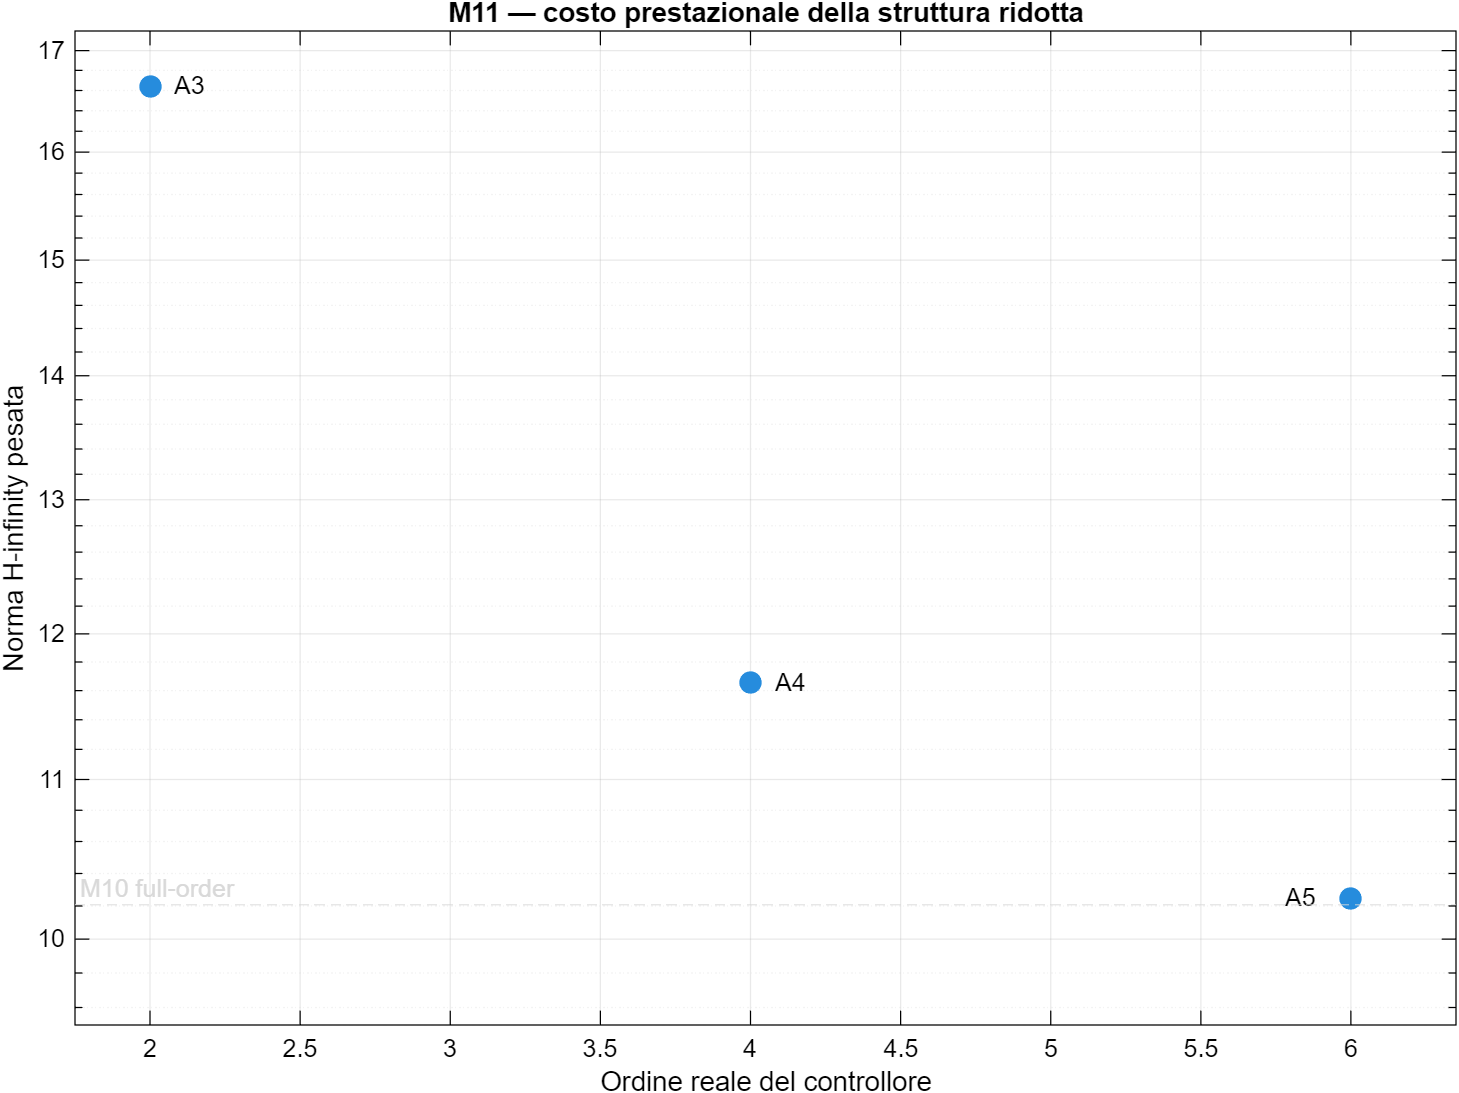
\includegraphics[width=0.80\textwidth]{figures/m11_gamma_vs_order.png}
\caption{Frontiera ordine--objective M11, rigenerata con i nuovi $W_1,W_2$.}
\label{fig:m11-order}
\end{figure}
A5, ordine 6, alimenta M12; non coincide con $K_\infty$ M10,
ordine 18. La tabella seguente deriva dagli artifact correnti.
% Tabella generata da build_m18_report_tables.m.
\begin{table}[H]
\centering
\begin{tabular}{lllll}
\toprule
Controllore & Ordine & $\gamma$/objective & NS & NP \\
\midrule
M9 mixsyn & 18 & 5.6772 & PASS & FAIL \\
M10 hinfsyn & 18 & 5.6772 & PASS & FAIL \\
M11 A3 & 2 & 8.1671 & PASS & FAIL \\
M11 A4 & 4 & 5.9672 & PASS & FAIL \\
M11 A5 & 6 & 5.7086 & PASS & FAIL \\
\bottomrule
\end{tabular}
\caption{Sintesi nominali H-infinity. Un valore $\gamma>1$ non costituisce PASS prestazionale.}
\label{tab:hinf}
\end{table}


\section{Risultati del nuovo studio e figure didattiche}
% Generated by plot_hinf_revision.m.
\begin{table}[htbp]\centering\small
\begin{tabular}{rrrrrrrr}\toprule
ID & $\omega_B$ & $\beta_U$ & $\omega_T$ & $\gamma$ & OS [\%] & picco $u$ & stabili/5 \\\midrule
0 & 12 & 11.459 & 0 & 10.207 & 261.62 & 5.1599 & 5 \\
1 & 12 & 1 & 0 & 3.4477 & 155.9 & 14.19 & 2 \\
2 & 8 & 1 & 40 & 2.8302 & 149.13 & 11.859 & 3 \\
3 & 8 & 1 & 80 & 2.8056 & 152.82 & 11.956 & 3 \\
4 & 8 & 2 & 40 & 3.6641 & 180.56 & 8.7844 & 4 \\
5 & 8 & 2 & 80 & 3.6476 & 186.15 & 8.829 & 4 \\
6 & 12 & 1 & 40 & 3.4886 & 145.41 & 13.952 & 3 \\
7 & 12 & 1 & 80 & 3.4624 & 151.62 & 14.069 & 2 \\
8 & 12 & 2 & 40 & 4.4659 & 175.43 & 10.222 & 3 \\
9 & 12 & 2 & 80 & 4.4561 & 180.17 & 10.297 & 3 \\
10 & 16 & 1 & 40 & 4.073 & 144.44 & 15.686 & 2 \\
11 & 16 & 1 & 80 & 4.0464 & 153.38 & 15.818 & 2 \\
12 & 16 & 2 & 40 & 5.1858 & 169.39 & 11.438 & 3 \\
13 & 16 & 2 & 80 & 5.1687 & 173.44 & 11.51 & 3 \\
\bottomrule\end{tabular}
\caption{Campagna deterministica. ID 0 è la baseline ricaricata; ID 1 isola la nuova scala di comando senza $W_3$. Le frequenze sono in rad/s, il comando in N m. Tutti sono nominalmente stabili; nessuno supera tutti i target M5. I cinque campioni M4 non certificano robustezza.}
\label{tab:hinf-campagna}\end{table}
\begin{table}[htbp]\centering\small
\begin{tabular}{lrr}\toprule
Metrica & M10 originale & candidato illustrativo \\\midrule
$\gamma$ & 10.207 & 4.073 \\
$\|W_1S\|_\infty$ & 10.128 & 4.0702 \\
$\|W_2KS\|_\infty$ & 10.185 & 4.0339 \\
$\|W_3T\|_\infty$ & 0 & 2.5921 \\
$T_s$ [s] & 1.566 & 1.162 \\
Overshoot [\%] & 261.62 & 144.44 \\
Errore statico relativo & 0.49068 & 0.20143 \\
Cross-coupling & 0.2596 & 0.19912 \\
Picco comando [N m] & 5.1599 & 15.686 \\
RMS comando [N m] & 1.0517 & 1.1913 \\
Ordine & 18 & 20 \\
\bottomrule\end{tabular}
\caption{Metriche peggiori fra due gradini nominali separati da 5 gradi, 12 s, senza disturbi o rumore. I valori $\gamma$ riguardano problemi pesati diversi: non sono direttamente una graduatoria di robustezza.}
\label{tab:hinf-nuovo-confronto}\end{table}

Nessuno dei 12 candidati è conforme. Il compromesso selezionato
riduce il costo pesato, ma conserva overshoot e offset elevati.
I valori completi provengono dalle tabelle generate: una riduzione
di $\gamma$ fra problemi con pesi differenti non è da sola una
graduatoria di robustezza.

% Generato da build_direct_weights_summary.m.
\begin{table}[htbp]\centering\scriptsize
\begin{tabular}{lrrrrrrrl}\toprule
Controllore & ordine & $\gamma$ & $\|W_1S\|_\infty$ & $\|W_2KS\|_\infty$ & $T_s$ & OS [\%] & picco $u$ & Esito \\
\midrule
M9 & 18 & 5.6772 & 5.6002 & 5.6568 & 1.486 & 228.62 & 9.5908 & FAIL \\
M10 & 18 & 5.6772 & 5.6002 & 5.6568 & 1.486 & 228.62 & 9.5908 & FAIL \\
M11 A3 & 2 & 8.1671 & 8.1473 & 8.1337 & 2.548 & 208.45 & 7.3041 & FAIL \\
M11 A4 & 4 & 5.9672 & 5.9602 & 5.9538 & 2.27 & 227.24 & 9.6453 & FAIL \\
M11 A5 & 6 & 5.7086 & 5.6336 & 5.6904 & 1.772 & 223.49 & 9.3331 & FAIL \\
\bottomrule\end{tabular}
\caption{Produzione a due pesi, senza $W_3$: scenari esistenti, tempi in s, coppie in N m. Esiti calcolati con soglie invariate.}\label{tab:direct-production}\end{table}
\begin{table}[htbp]\centering\small
\begin{tabular}{lrr}\toprule Controllore & errore statico relativo & cross-coupling \\
\midrule
M9 & 0.815096 & 0.244732 \\
M10 & 0.815096 & 0.244732 \\
M11 A3 & 1.18556 & 0.745547 \\
M11 A4 & 0.888898 & 0.32632 \\
M11 A5 & 0.841834 & 0.233384 \\
\bottomrule\end{tabular}\caption{Metriche relative della stessa campagna; il target statico rimane 0.05.}\end{table}

La tabella della produzione riporta gli scenari M9/M10/M11 esistenti:
il picco peggiore comprende anche il gradino da 8 gradi, mentre lo
studio dei pesi usa due gradini da 5 gradi. I valori non vanno confusi.

La Figura~\ref{fig:hinf-pesi-rivisti} mostra le modifiche ai pesi.
La Figura~\ref{fig:hinf-inviluppi} risponde invece alla domanda
se le due direzioni singolari di $S$ e $T$ rispettino gli inviluppi
scelti. Il confronto scalare è corretto perché ogni peso è un filtro
scalare replicato sui due canali, non una matrice arbitraria.
\begin{figure}[htbp]\centering
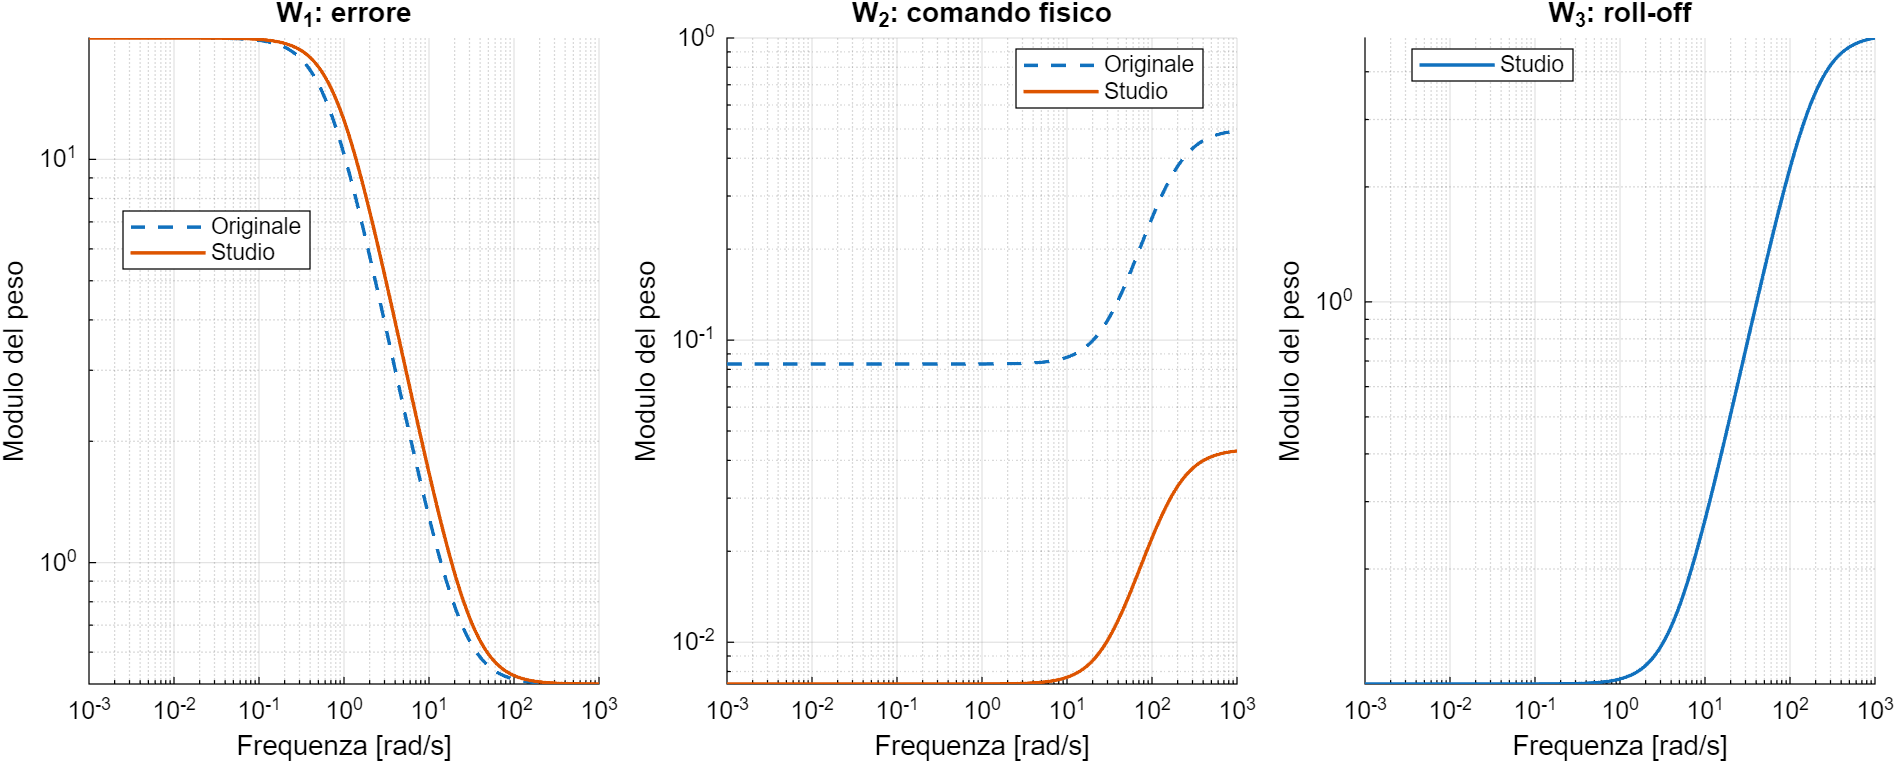
\includegraphics[width=0.98\textwidth]{figures/hinf_revision_weights.png}
\caption{Pesi fisici originali e del candidato ID 10. Il vecchio $W_3$ è assente, non un filtro non nullo nascosto sotto il grafico.}
\label{fig:hinf-pesi-rivisti}
\end{figure}
\begin{figure}[htbp]\centering
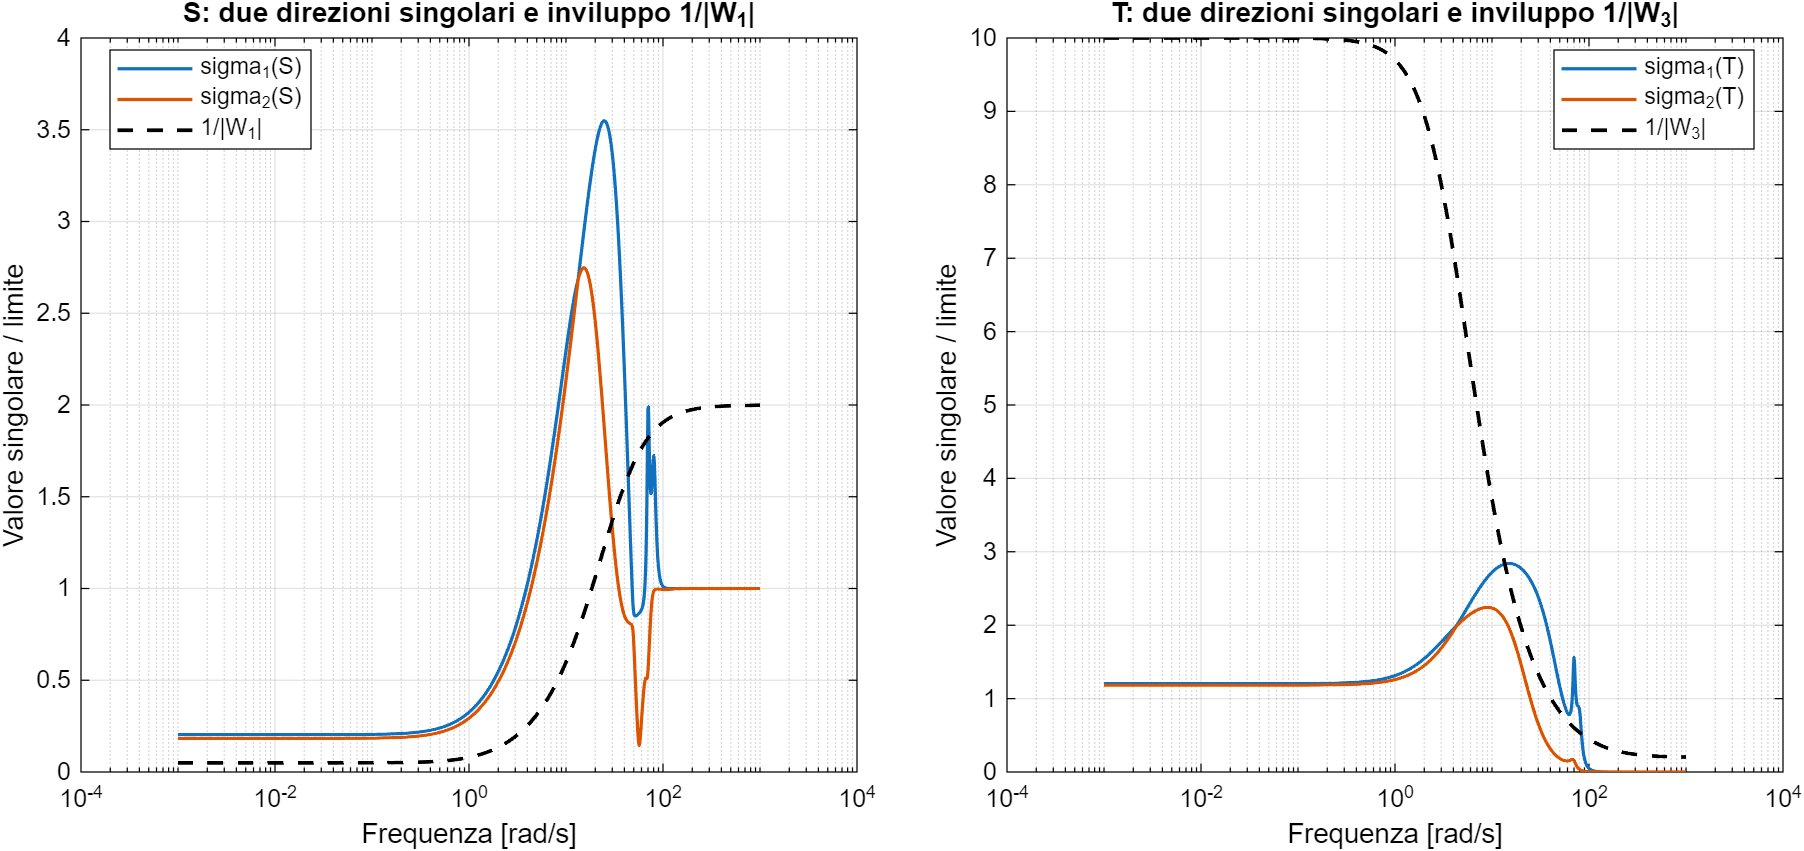
\includegraphics[width=0.96\textwidth]{figures/hinf_revision_sensitivity_envelopes.png}
\caption{Valori singolari di $S$ e $T$ confrontati rispettivamente con $1/|W_1|$ e $1/|W_3|$. Gli inviluppi sono obiettivi del nuovo problema, non certificati di robustezza.}
\label{fig:hinf-inviluppi}
\end{figure}

La Figura~\ref{fig:hinf-canali-rivisti} espone direttamente i tre
contributi e il livello uno. La norma dello stack non è semplicemente
il massimo delle tre norme: i canali si sommano quadraticamente
nella matrice prestazionale prima della massimizzazione.
\begin{figure}[htbp]\centering
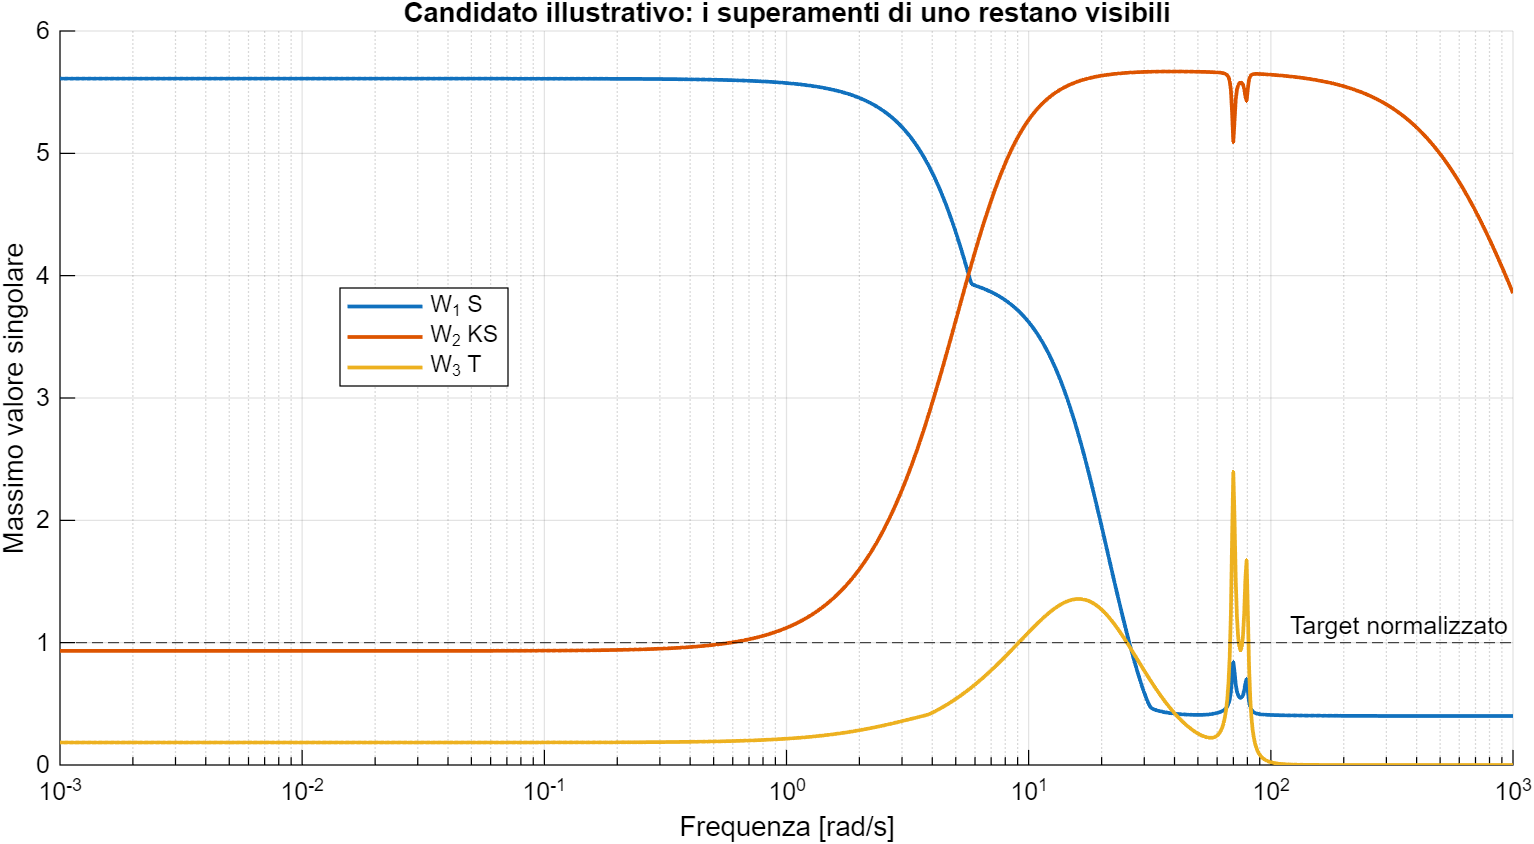
\includegraphics[width=0.72\textwidth]{figures/hinf_revision_weighted_channels.png}
\caption{Massimi valori singolari di $W_1S$, $W_2KS$, $W_3T$ per ID 10. Tutti i superamenti del target sono conservati.}
\label{fig:hinf-canali-rivisti}
\end{figure}
La Figura~\ref{fig:hinf-tempo-rivisto} mostra due esperimenti separati
con stesso orizzonte di 12 s, stato nullo, nessun disturbo o rumore.
Le colonne distinguono il giunto di riferimento, le righe posizioni
e comandi. L'overshoot molto elevato e l'offset finale spiegano
perché il risultato resti un compromesso non conforme, pur essendo
stati adottati i suoi pesi nella revisione della catena di produzione.
\begin{figure}[!htbp]\centering
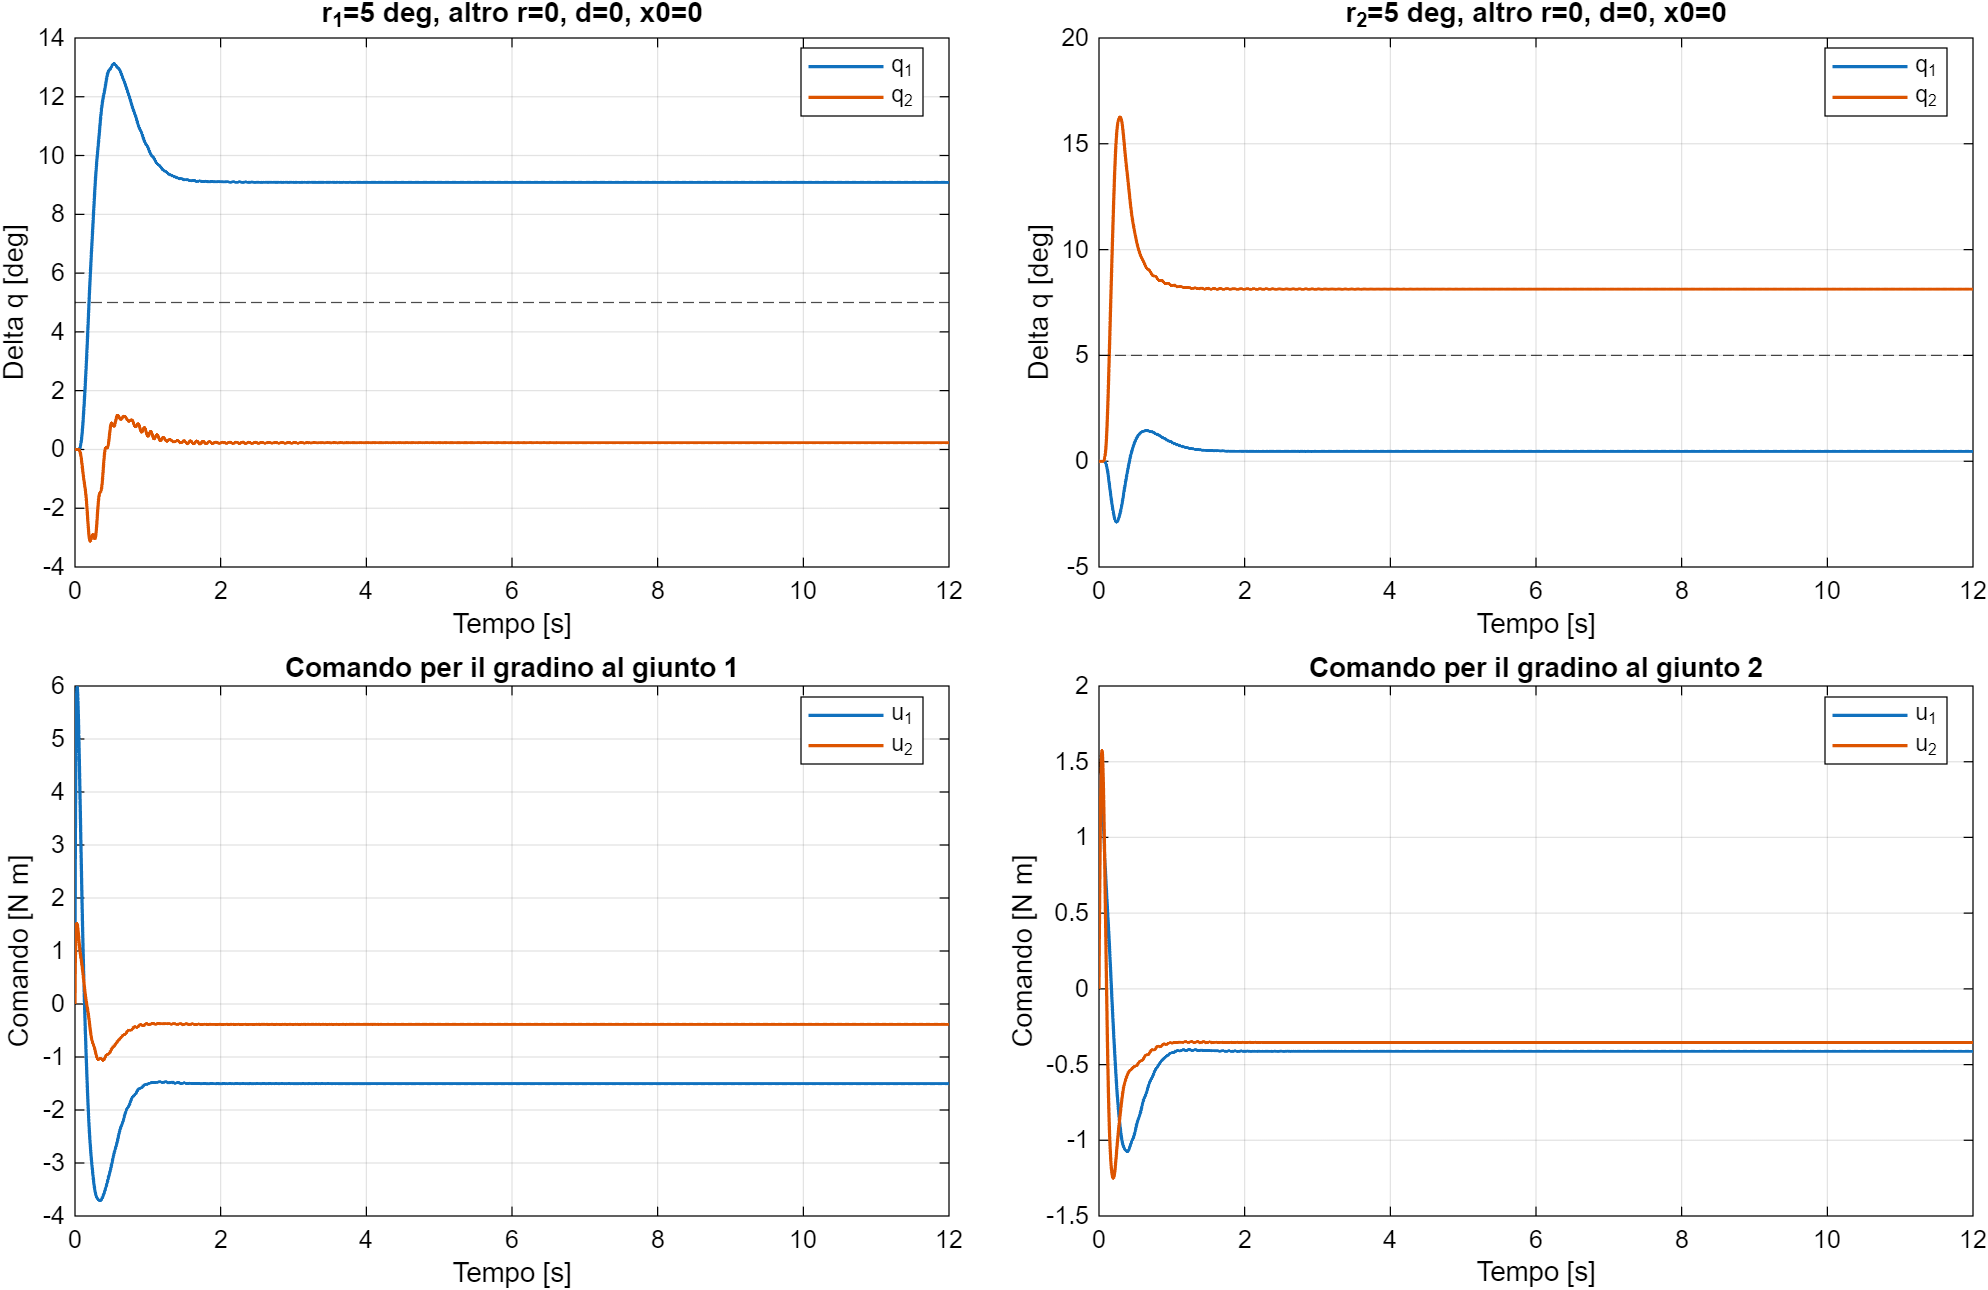
\includegraphics[width=0.78\textwidth]{figures/hinf_revision_tracking_control.png}
\caption{Tracking e comando di ID 10 per gradini da 5 gradi. La linea tratteggiata indica il riferimento del giunto eccitato; l'altro riferimento è nullo. Nessun prefiltro o saturazione è aggiunto.}
\label{fig:hinf-tempo-rivisto}
\end{figure}

La catena direttamente dipendente viene rigenerata: M12 sul nuovo A5,
M13 sul nuovo problema incerto pesato, M14 sul nuovo $K_\mu$ e
le validazioni M15--M17 sui controllori correnti.
M0--M4, criteri e scenari rimangono invariati.
La sintesi nominale $H_\infty$ non sostituisce la $\mu$-analysis;
M16 resta evidenza empirica e non certificazione di robustezza.
